\subsection{by Radoslaw Lojek}

\subsubsection{Introduction}
The solution I have designed is the most intuitive and straight forward algorithm. It checks all
possible elements along its way. If a domino piece satisfies necessary conditions of being removed,
it is thrown away from a board of elements. The operation is repeated for all consecutive elements
until nothing can't be removed, or the domino board is empty.

\subsubsection{Data structure}
The data structure I have decided to use is a two dimensional array of objects, where object is a
single domino field. Each object consists of fields such as: its value, location X and Y, boolean
saying if a piece is placed horizontally/vertically, boolean saying if it is successor or
predecessor field (value above or on the left side of a domino piece is successor, otherwise
predecessor) and of course pointer to the other half of the piece. If a single cell in a matrix is
empty, meaning that no piece is there, it is marked as a null pointer.
\\
\begin{minted}[linenos,numbersep=5pt]{c++}
class dominoField {
   int value;
   int X;
   int Y; 
   boolean isSuccessor;
   boolean isVertical; 
   dominoField *twinField; 
}
\end{minted}


\subsubsection{Algorithm Pseudo-Code}
The algorithm takes as a parameters two dimensional array of elements and its vertical and
horizontal size. Returns elements that were removed during the calculations. Below algorithm is
simple, since it does not involve more complicated concepts such as Artificial Intelligence or
complex graph algorithms.
\\
\begin{minted}[linenos,numbersep=5pt]{c++}
List<dominoPiece> solveDominoProblem(dominoField **board, int dimX, int dimY){
   List<dominoPiece> result_list;
   int iterPiecesRemoved = 1;
   
   while iterPiecesRemoved != 0 {
      iterPiecesRemoved = 0;
      for i = 0 to dimX {
         for j = 0 to dimY {
            if !isEmpty(board,i,j) and isElemRemovable(board, dimX, dimY, i, j){ 
               result_list.add( removePiece(board,i,j) );
               iterPiecesRemoved = iterPiecesRemoved + 1;
            }
         }
      }
   }
   return result_list;
}
\end{minted}

%\begin{wrapfigure}{r}{0.3\textwidth}
%  \vspace{-30pt}
  \begin{center}
    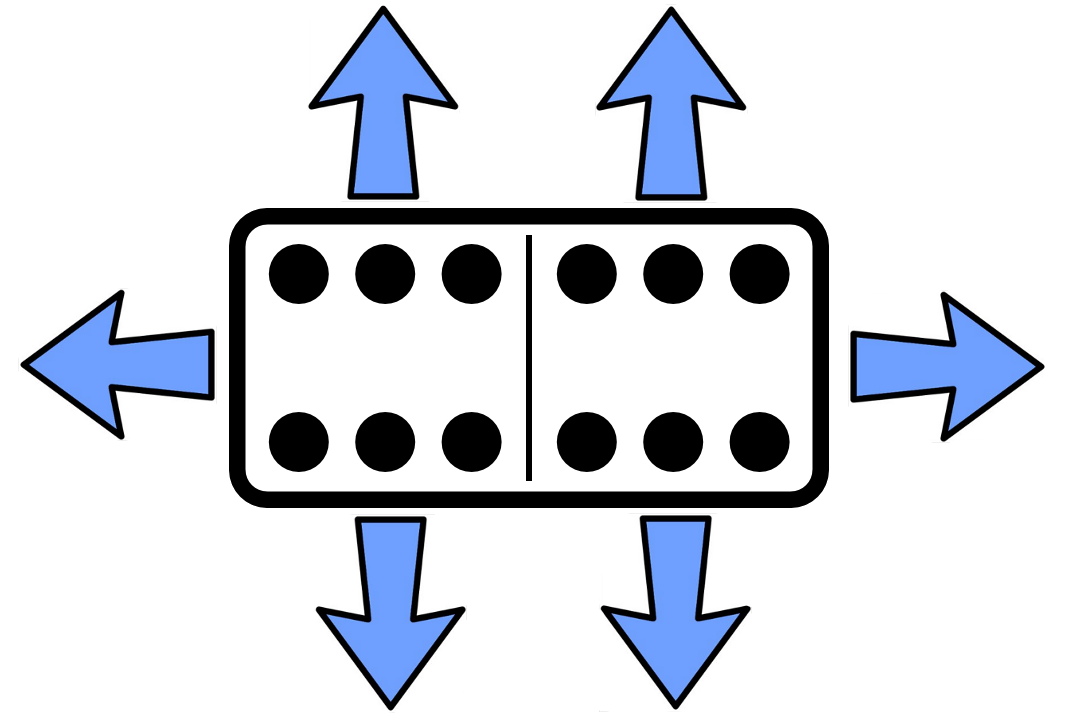
\includegraphics[width=0.2\textwidth]{dirPiece.png}
  \end{center}
 % \vspace{-20pt}
%\end{wrapfigure}

I will let myself omit pseudo code of functions used above. Just briefly explain how isElemRemovable
will work: depending on the location of a 'twinField' of a single piece, function counts the number
of empty fields in each possible direction (as depicted on the right). Once the directions are
counted, function checks if they meet requirements for the piece to be removed - if it does, returns
true or false otherwise.

\subsubsection{Time complexity}
Time complexity of the considered algorithm is \textit{$n^2$}, since we go in each iteration 
through all possible domino fields \textit{n} times. Each iteration is repeated in worst case
\textit{1/2*n} times, because may occur situation in which only one domino element (two fields)
disappears in one \textit{while} loop iteration.

\subsubsection{Example}

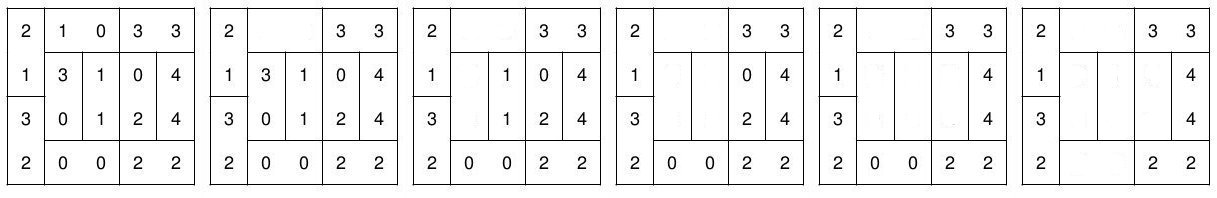
\includegraphics[width=1\textwidth]{board1.jpg} \\
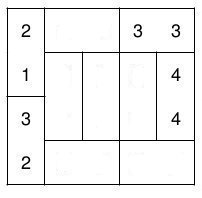
\includegraphics[width=0.163\textwidth]{board2.jpg}
